% algorithmes de plus courts chemins 

\begin{frame}{Graphes pondérés}

\begin{definition}
    Un graphe \emph{non-orienté pondéré} est un graphe non-orienté muni d'une fonction de pondération qui associe une valeur réelle à chaque arête. 
\end{definition}

\begin{definition}
    Un graphe \emph{orienté pondéré} est un graphe orienté muni d'une fonction de pondération qui associe une valeur réelle à chaque arc. 
\end{definition}

\end{frame}

\begin{frame}{Exemple : graphe non-orienté pondéré}
    \begin{center}
        \begin{tikzpicture}
\clip (0,0) rectangle (6,6);
\Vertex[x=0.450,y=5.550,size=0.8,opacity=0.5,label=1]{0}
\Vertex[x=0.450,y=3.000,size=0.8,opacity=0.5,label=2]{1}
\Vertex[x=3.000,y=3.000,size=0.8,opacity=0.5,label=3]{2}
\Vertex[x=3.000,y=5.550,size=0.8,opacity=0.5,label=4]{3}
\Vertex[x=5.550,y=5.550,size=0.8,opacity=0.5,label=5]{4}
\Vertex[x=5.550,y=3.000,size=0.8,opacity=0.5,label=6]{5}
\Vertex[x=5.550,y=0.450,size=0.8,opacity=0.5,label=7]{6}
\Vertex[x=3.000,y=0.450,size=0.8,opacity=0.5,label=8]{7}
\Vertex[x=0.450,y=0.450,size=0.8,opacity=0.5,label=9]{8}
\Edge[,lw=2.0,bend=-8.531,label=5](0)(1)
\Edge[,lw=2.0,bend=-8.531,label=2](0)(3)
\Edge[,lw=2.0,bend=-8.531,label=-2](1)(3)
\Edge[,lw=2.0,bend=-8.531,label=4](2)(8)
\Edge[,lw=2.0,bend=-8.531,label=1](4)(5)
\Edge[,lw=2.0,bend=-8.531,label=3](5)(6)
\Edge[,lw=2.0,bend=-8.531,label=0](6)(7)
\end{tikzpicture}

    \end{center}
    \end{frame}

% TODO exemple de graphe orienté avec pondération ?

\begin{frame}{Applications}
    \begin{itemize}
        \item Calcul de plus courts chemins 
        \begin{itemize}
            \item Distances entre villes
        \end{itemize}
        \item Arbres couvrants minimaux 
        \item Contraintes entre tâches 
    \end{itemize}
\end{frame}

\begin{frame}{Arbre couvrant}
    \begin{definition}
        Dans un graphe $G$ non orienté (pondéré ou non) connexe, un arbre couvrant est un sous-graphe connexe acyclique (arbre) incluant tous les sommets de $G$
    \end{definition}


\end{frame}

% TODO ajouter définition d'un sous-graphe 


\begin{frame}{Exemple : arbre couvrant}
    \begin{center}
        \begin{tikzpicture}
\clip (0,0) rectangle (6,6);
\Vertex[x=0.450,y=5.550,size=0.8,opacity=0.5,label=1]{0}
\Vertex[x=0.450,y=3.000,size=0.8,opacity=0.5,label=2]{1}
\Vertex[x=3.000,y=3.000,size=0.8,opacity=0.5,label=3]{2}
\Vertex[x=3.000,y=5.550,size=0.8,opacity=0.5,label=4]{3}
\Vertex[x=5.550,y=5.550,size=0.8,opacity=0.5,label=5]{4}
\Vertex[x=5.550,y=3.000,size=0.8,opacity=0.5,label=6]{5}
\Vertex[x=5.550,y=0.450,size=0.8,opacity=0.5,label=7]{6}
\Vertex[x=3.000,y=0.450,size=0.8,opacity=0.5,label=8]{7}
\Vertex[x=0.450,y=0.450,size=0.8,opacity=0.5,label=9]{8}
\Edge[,lw=2.0,bend=-8.531](0)(1)
\Edge[,lw=4.0,bend=-8.531](0)(3)
\Edge[,lw=4.0,bend=-8.531,](1)(3)
\Edge[,lw=4.0,bend=-8.531](2)(8)
\Edge[,lw=4.0,bend=-8.531](4)(5)
\Edge[,lw=4.0,bend=-8.531](5)(6)
\Edge[,lw=4.0,bend=-8.531](6)(7)
\Edge[,lw=4.0,bend=-8.531](3)(4)
\Edge[,lw=4.0,bend=-8.531](2)(6)
\Edge[,lw=2.0,bend=-8.531](2)(1)
\end{tikzpicture}

    \end{center}
    \end{frame}

    \begin{frame}{Contre-exemple : arbre non couvrant}
        \begin{center}
            \begin{tikzpicture}
\clip (0,0) rectangle (6,6);
\Vertex[x=0.450,y=5.550,size=0.8,opacity=0.5,label=1]{0}
\Vertex[x=0.450,y=3.000,size=0.8,opacity=0.5,label=2]{1}
\Vertex[x=3.000,y=3.000,size=0.8,opacity=0.5,label=3]{2}
\Vertex[x=3.000,y=5.550,size=0.8,opacity=0.5,label=4]{3}
\Vertex[x=5.550,y=5.550,size=0.8,opacity=0.5,label=5]{4}
\Vertex[x=5.550,y=3.000,size=0.8,opacity=0.5,label=6]{5}
\Vertex[x=5.550,y=0.450,size=0.8,opacity=0.5,label=7]{6}
\Vertex[x=3.000,y=0.450,size=0.8,opacity=0.5,label=8]{7}
\Vertex[x=0.450,y=0.450,size=0.8,opacity=0.5,label=9]{8}
\Edge[,lw=2.0,bend=-8.531](0)(1)
\Edge[,lw=4.0,bend=-8.531](0)(3)
\Edge[,lw=4.0,bend=-8.531,](1)(3)
\Edge[,lw=4.0,bend=-8.531](2)(8)
\Edge[,lw=2.0,bend=-8.531](4)(5)
\Edge[,lw=4.0,bend=-8.531](5)(6)
\Edge[,lw=4.0,bend=-8.531](6)(7)
\Edge[,lw=4.0,bend=-8.531](3)(4)
\Edge[,lw=4.0,bend=-8.531](2)(6)
\Edge[,lw=2.0,bend=-8.531](2)(1)
\end{tikzpicture}

        \end{center}
        \end{frame}
    
\begin{frame}{Construction d'un arbre couvrant}
\begin{itemize}
    \item Connaissez-vous un algorithme capable de construire un arbre couvrant ?
    \pause \item Oui !
    \pause \item Tous les algorithmes de parcours que nous avons vus jusqu'ici 
    \pause \item Pour de bonnes raisons applicatives, on va chercher à construire un arbre couvrant \emph{minimal} 
    \pause \item Est-on obligés de parcourir l'ensemble des arbres couvrants pour trouver un arbre de coût minimal ?
\end{itemize}
    
\end{frame}

\begin{frame}{Applications}
    \begin{itemize}
        \item Minimiser la longueur de câble nécessaire pour connecter un réseau 
        \item Heuristique dans certains problèmes d'optimisation
        \begin{itemize}
            \item problème du voyageur de commerce
        \end{itemize}
    \end{itemize}
\end{frame}

\begin{frame}{Arbre couvrant minimal}
    \begin{definition}
        Dans un graphe non orienté pondéré et connexe, un arbre couvrant minimal est un arbre couvrant dont la somme des arêtes est minimale
    \end{definition}

    \begin{itemize}
        \item Remarque : si le graphe n'est pas pondéré, on considère des arêtes de poids identique 
    \end{itemize}
\end{frame}

\begin{frame}{Exemple 1 : arbre couvrant minimal (non pondéré)}
    \begin{center}
        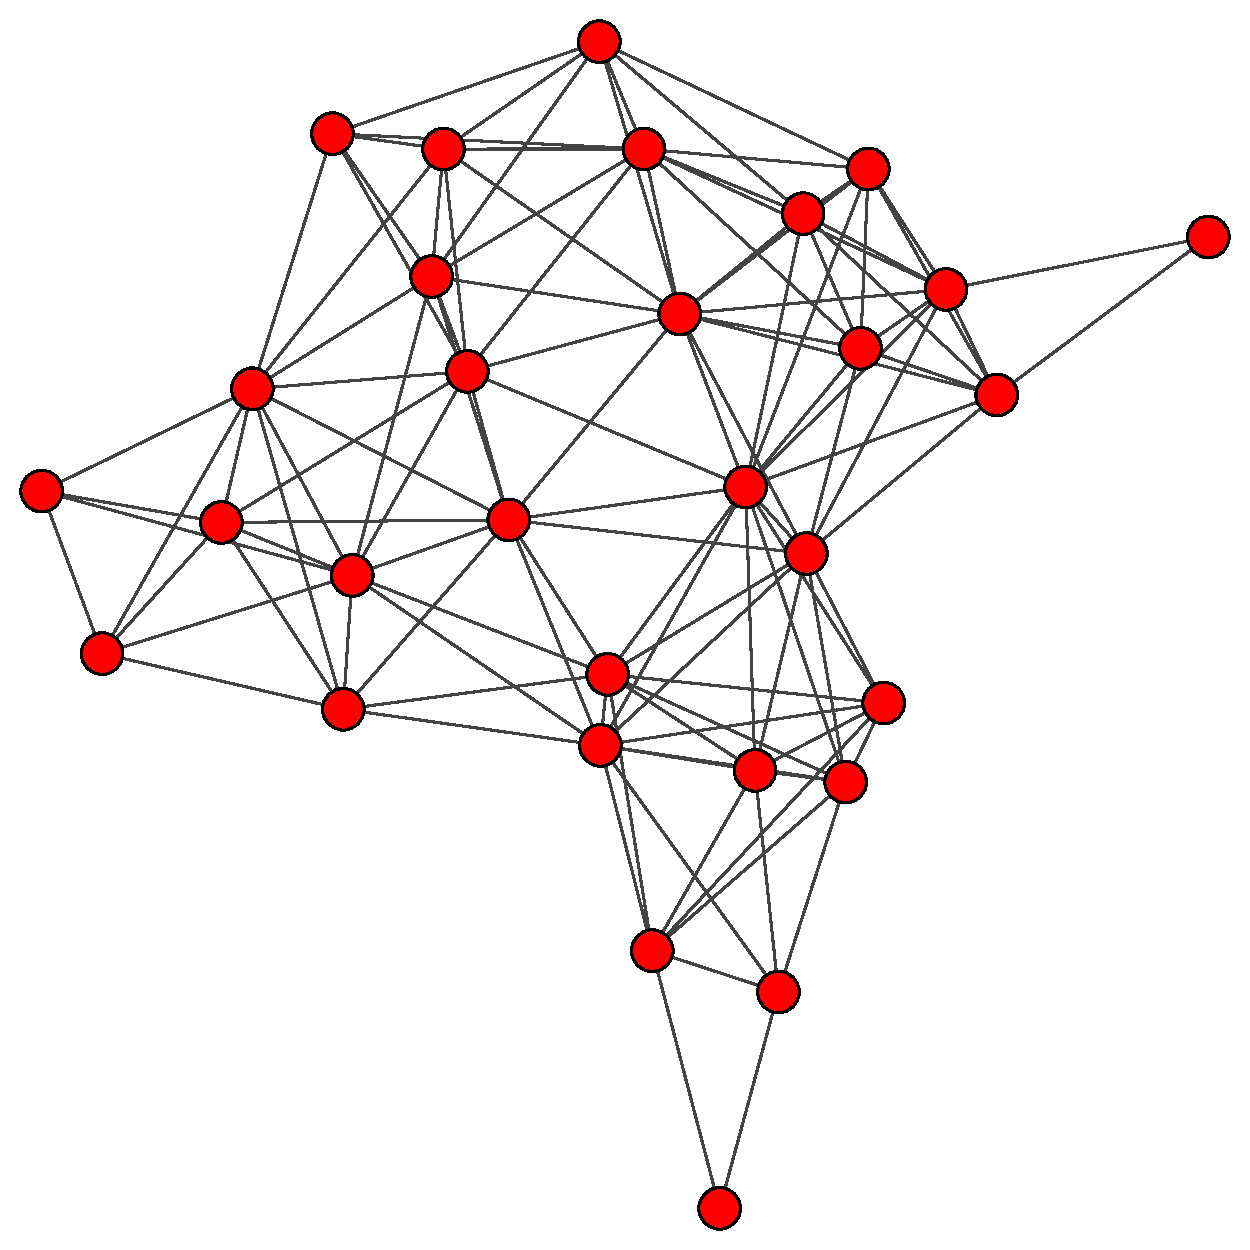
\includegraphics[height=.8\textheight]{fig/mst-0.pdf}
    \end{center}
\end{frame}
\begin{frame}{Exemple 1 : arbre couvrant minimal (non pondéré)}
    \begin{center}
        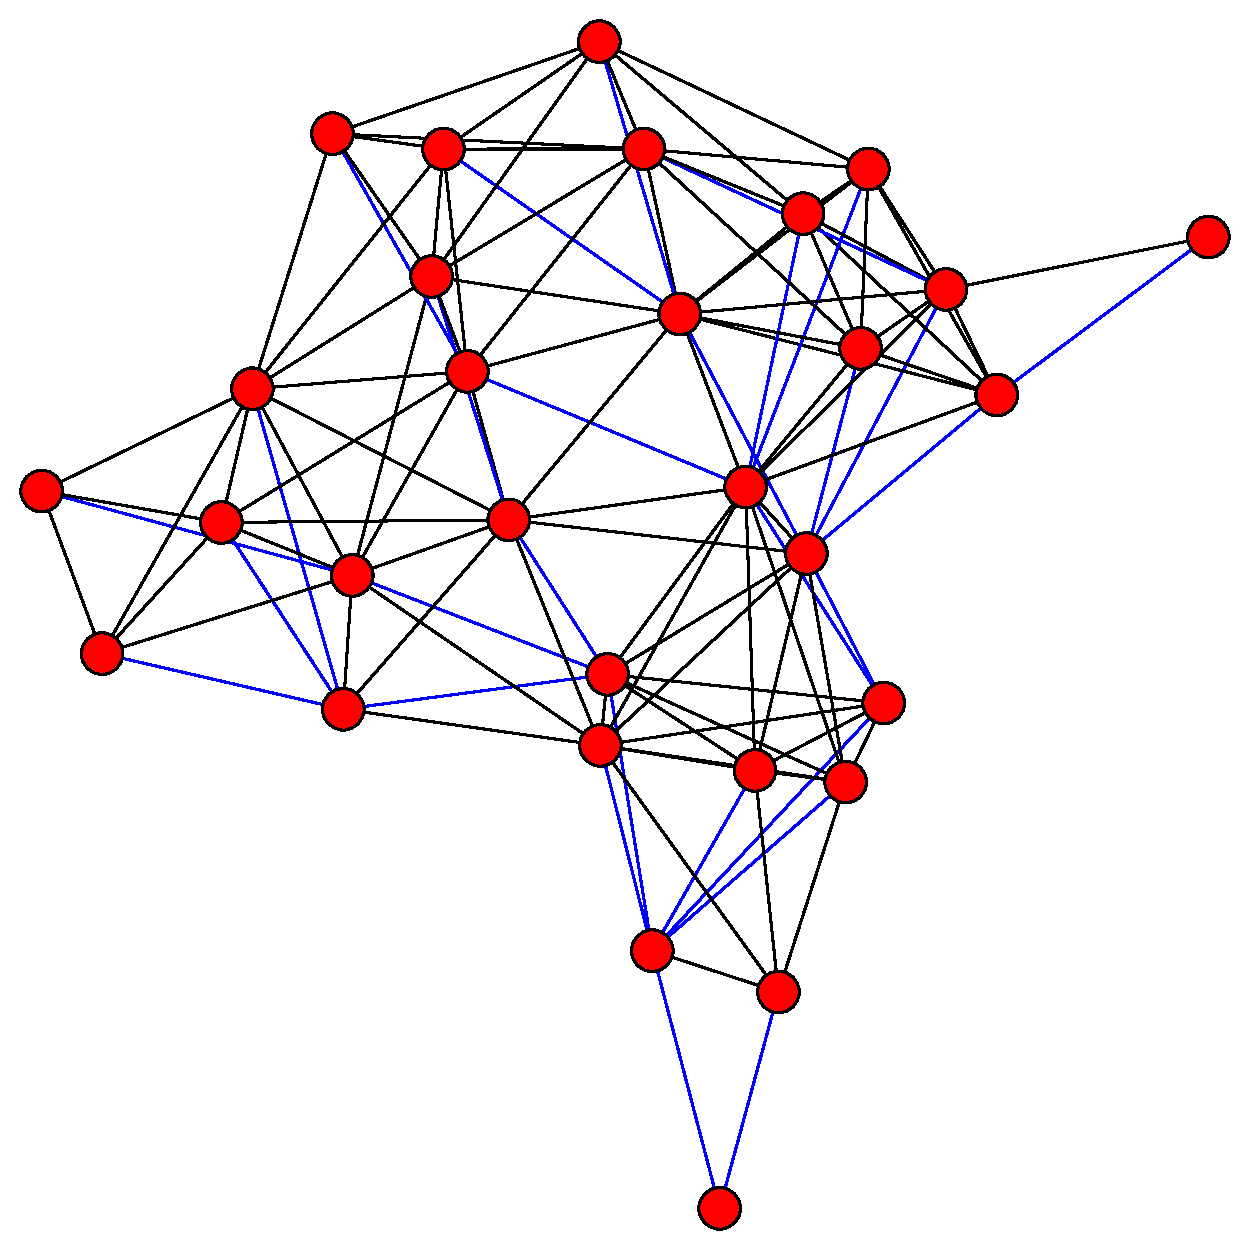
\includegraphics[height=.8\textheight]{fig/mst-1.pdf}
    \end{center}
\end{frame}
\begin{frame}{Exemple 1 : arbre couvrant minimal (non pondéré)}
    \begin{center}
        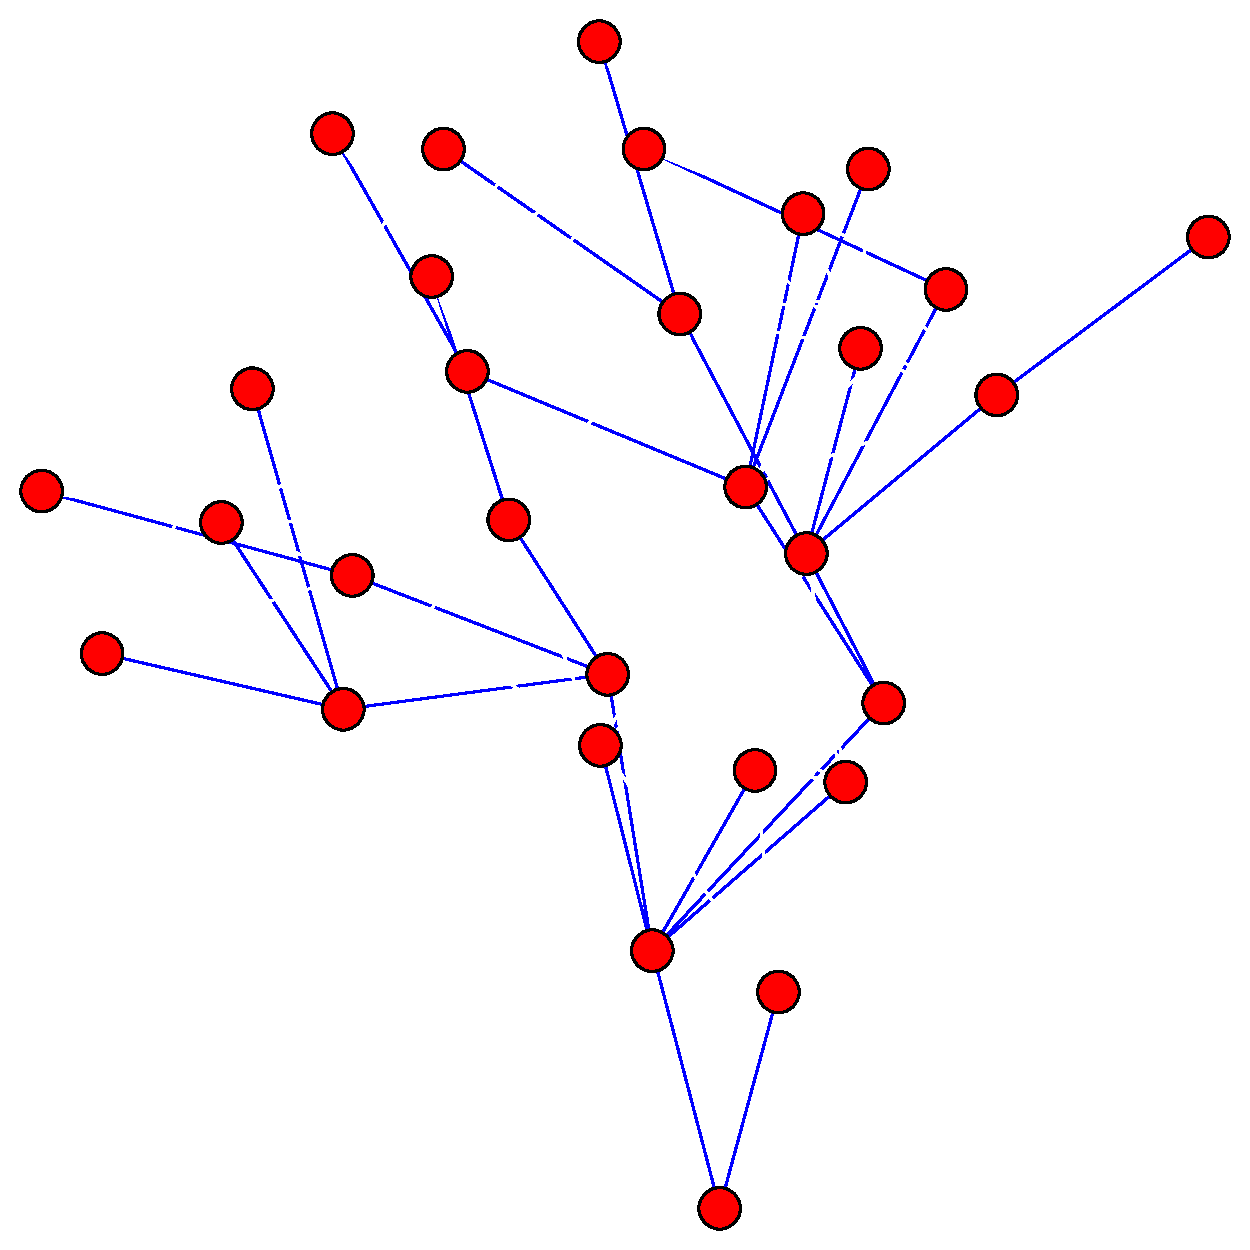
\includegraphics[height=.8\textheight]{fig/mst-2.pdf}
    \end{center}
\end{frame}

\begin{frame}{Exemple 2 : arbre couvrant minimal (pondéré)}
    \begin{center}
        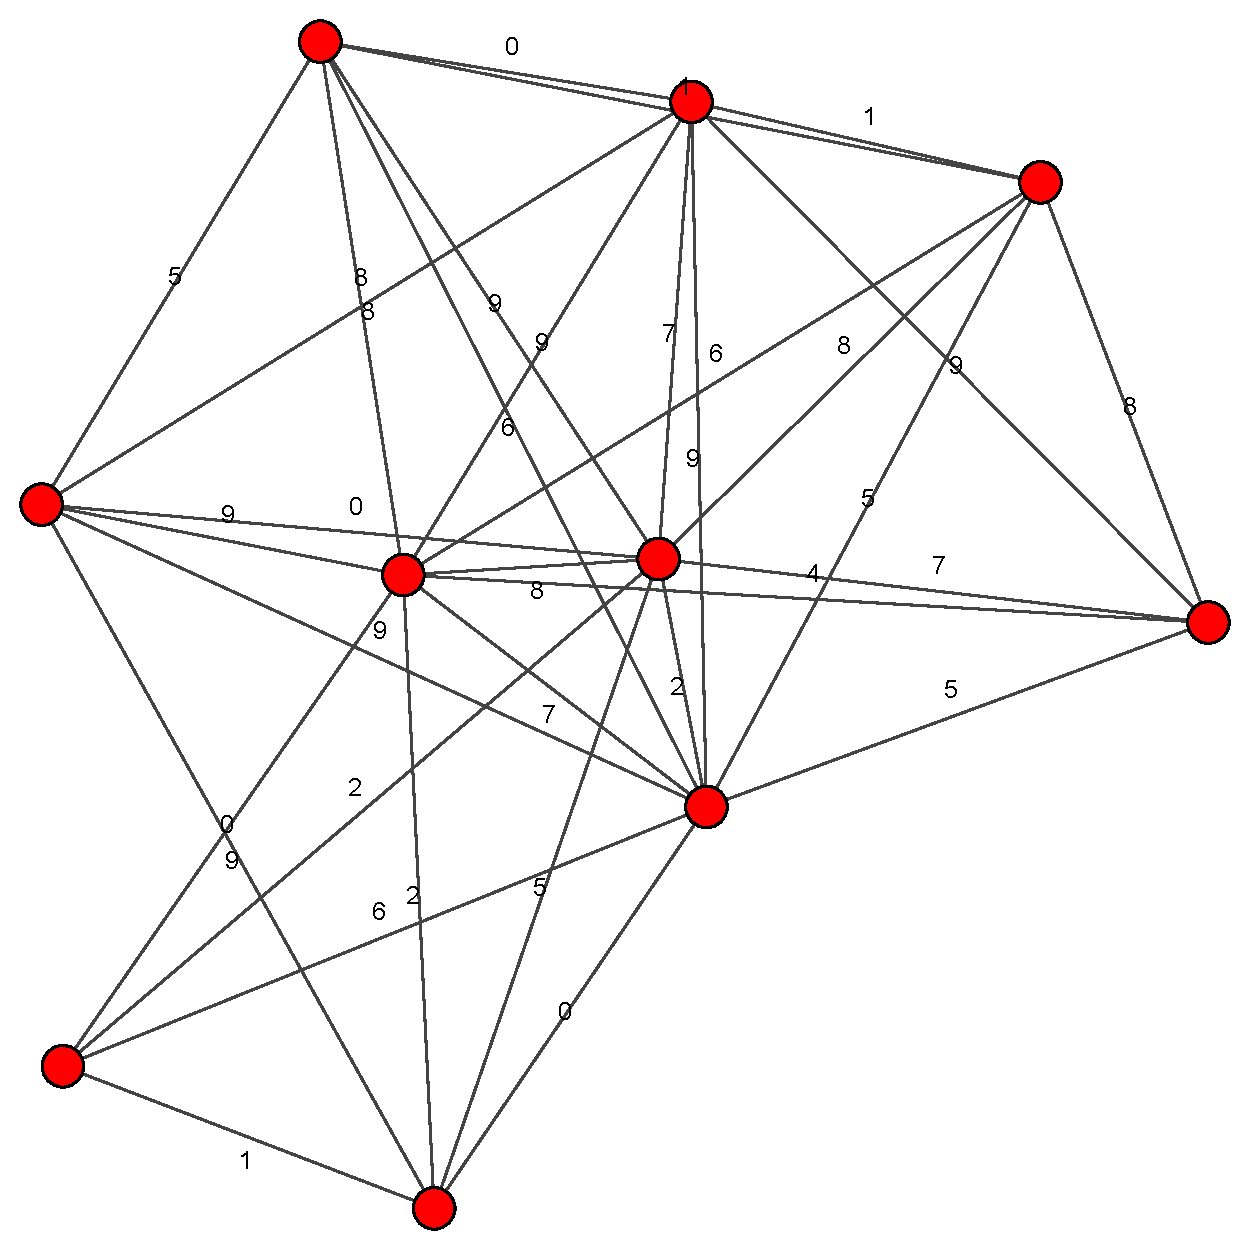
\includegraphics[height=.8\textheight]{fig/mstp-0.pdf}
    \end{center}
\end{frame}
\begin{frame}{Exemple 2 : arbre couvrant minimal (non pondéré)}
    \begin{center}
        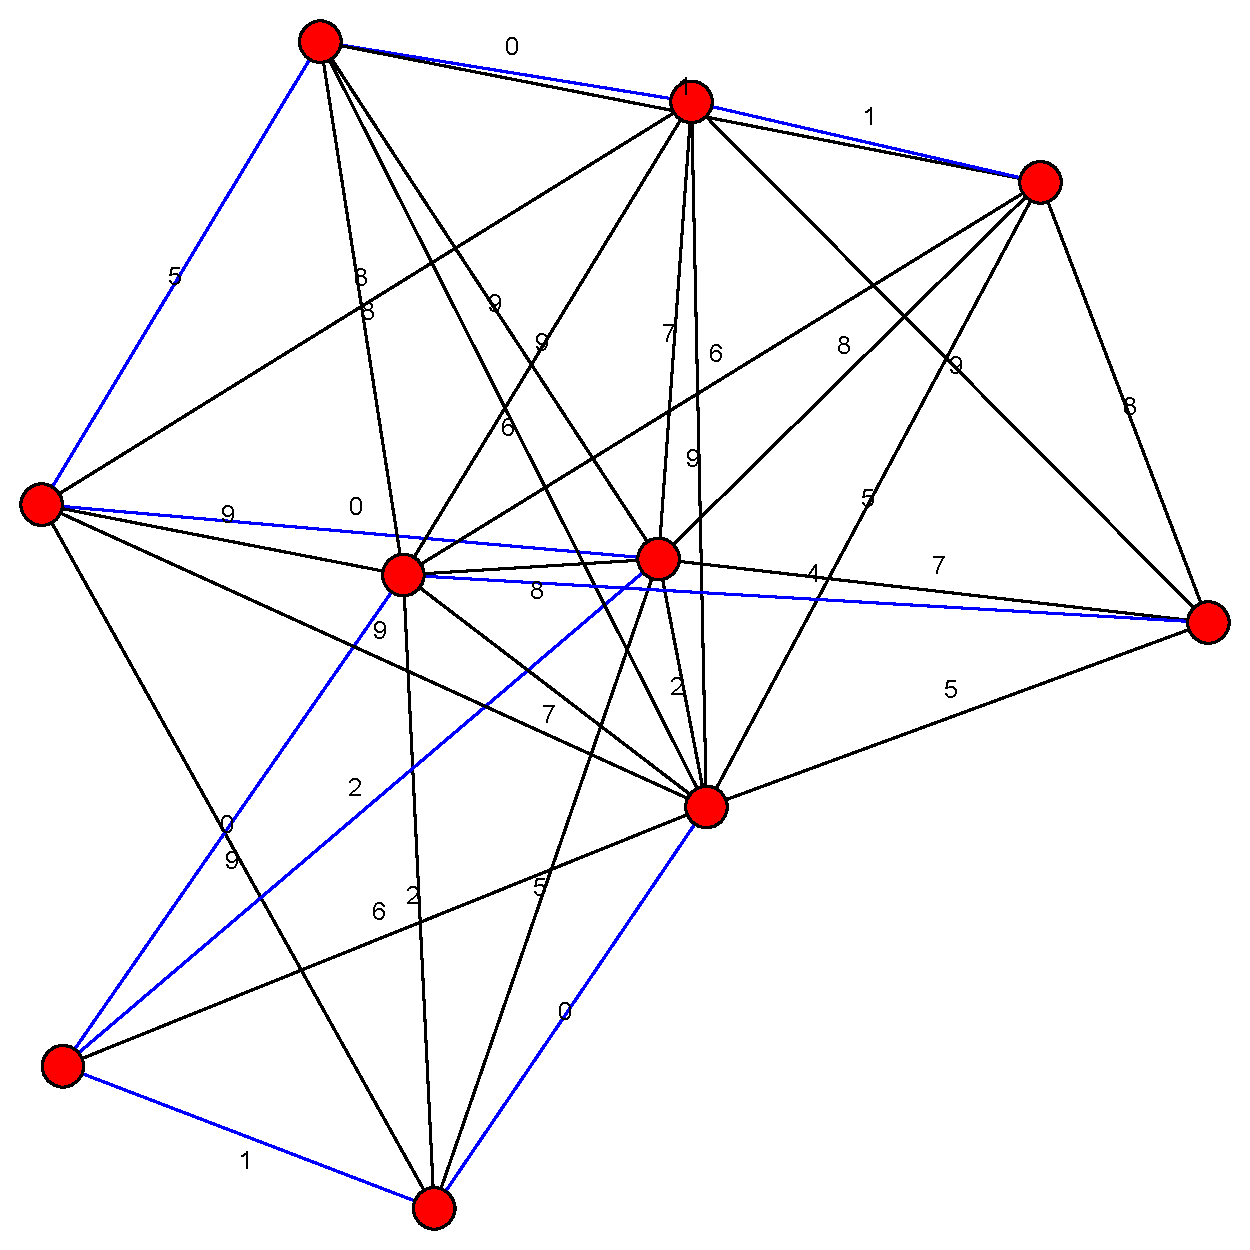
\includegraphics[height=.8\textheight]{fig/mstp-1.pdf}
    \end{center}
\end{frame}

\begin{frame}{Quelques ropriétés}
    \begin{block}{Propriété}
        Ajouter une arête à un graphe non-orienté connexe, crée un cycle
    \end{block}
    L'arête $a$ ajoutée connecte deux sommets $i$ et $j$. Or, le graphe étant connexe, il existait un chemin entre $i$ et $j$ dans le graphe initial. Ajouter $a$ à ce chemin crée un cycle.  
\end{frame}

\begin{frame}{Quelques propriétés}
    \begin{block}{Propriété}
        Enlever une arête à un arbre le rend non-connexe. L'arbre a alors exactement deux composantes connexes. 
    \end{block}
    On note $T-a$ l'arbre privé d'une arête quelconque $a$. On le suppose toujours connexe. Si on ajoute $a$ et qu'on applique la propriété précédente, $T-a$ auquel on a ajouté possède un cycle, ce qui est contradictoire avec le fait que $T$ est un arbre. 
\end{frame}

\begin{frame}{Coupe}
    \begin{definition}
        Une coupe associée à un graphe $G=(S,A)$ est une partition de l'ensemble des sommets $S$ en deux ensembles disjoints $S_1$ et $S_2$. Une arête traversante est une arête $(i,j)$ telle que $i \in S_1$ et $j \in S_2$. 
    \end{definition}
\end{frame}

\begin{frame}{Propriété des cycles}

    \begin{block}{Hypothèse}
        On considère un graphe non-orienté pondéré connexe. On suppose que toutes ses arêtes ont des poids différents
    \end{block}

    Cela assure l'unicité d'un arbre couvrant minimal (admis). Les algorithmes que nous allons voir n'ont pas besoin de cette hypothèse mais l'arbre couvrant minimal n'est plus unique. 
    
    \begin{block}{Propriété}
        Soit $C$ un cycle de $G$. Soit une $f$ une arête de poids maximum dans ce cycle. Alors $f$ n'appartient pas à l'arbre couvrant minimal.
    \end{block}

\end{frame}

\begin{frame}{Démonstration}

    \begin{itemize}
        \item Supposons, par l'absurde que $f$ appartienne à l'arbre couvrant minimal ACM
        \item Enlever $f$ de ACM le coupe en deux composantes connexes 
        \item Il existe une arête $e$ du cycle $C$ qui peut reconnecter les deux composantes 
        \item ACM$-{f}+{e}$ est un nouvel arbre couvrant 
        \item Comme $f$ était l'arête de poids maximum de $C$, ACM$-{f}+{e}$ a un poids inférieur strictement à ACM
        \item Contradiction !
    \end{itemize}
    
\end{frame}

\begin{frame}{Propriété de la coupe}
    
    \begin{block}{Propriété}
        Soit une coupe $S_1,S_2$ de $G$. Soit $e$ l'arête traversante de poids minimum de cette coupe. Alors $e$ appartient forcément à l'arbre couvrant minimal. 
    \end{block}
\end{frame}

\begin{frame}{Démonstration}
    \begin{itemize}
        \item On suppose, par l'absurde, que $e$ n'appartienne pas à l'ACM 
        \item Ajouter $e$ à l'ACM crée alors un cycle 
        \item Il existe une autre arête traversante $f$ qui sépare l'ACM en deux composantes connexes 
        \item ACM$-{f}+{e}$ est nouvel arbre couvrant 
        \item Son poids total est strictement inférieur à celui de ACM 
        \item Contradiction !
    \end{itemize}
\end{frame}


\begin{frame}{Schéma d'un algorithme glouton}
    \begin{itemize}
        \item On colorie toutes les arêtes de $G$ en noir. On va progressivement colorier en rouge les arêtes de l'arbre couvrant minimal 
        \item On choisit une coupe avec aucune arête traversante rouge 
        \item On sélectionne l'arête traversante de poids minimum et on la colorie en rouge 
        \item On répète jusqu'à avoir obtenu l'ACM. Combien d'arêtes faut-il ? 
        \begin{itemize}
            \item l'arbre couvrant minimal comporte $n-1$ arêtes 
        \end{itemize}
    \end{itemize}
\end{frame}

\begin{frame}{Correction de l'algorithme}
    \begin{itemize}
        \item Par propriété de la coupe, toutes les arêtes rouges sont dans ACM 
        \item Tant qu'il y a moins de $n-1$ arêtes rouges, on pourra toujours trouver une coupe 
        \begin{itemize}
            \item tant que la forêt noire n'est pas couvrante, ou pas connexe 
        \end{itemize}
    \end{itemize}
\end{frame}

\directlua{\detokenize{
    for i=1,8,1 do
        tex.sprint("\\begin{frame}{Exemple}\\begin{center} \\includegraphics[height=.8\\textheight]{fig/mst-greedy-", i, ".pdf} \\end{center} \\end{frame}")
    end
}}

\begin{frame}{Les algoroithmes gloutons}
    \begin{itemize}
        \item Approche algorithmique générale pour résoudre des problèmes d'optimisation 
        \item Construction progressive d'une solution 
        \item A chaque étape on fait un choix local optimal, sans se préoccuper de l'effet global
        \item L'approche gloutonne ne fonctionne pas toujours... mais reste simple 
    \end{itemize}
\end{frame}



\begin{frame}{Algorithme de Prim}
    \label{def:prim}
    \begin{itemize}
        \item On colorie toutes les arêtes de $G$ en noir. Puis on va progressivement colorier en rouge les arêtes de l'arbre couvrant minimal. A chaque étape le sous-graphe rouge est un arbre. On colorie en rouge les sommets reliés par des arêtes rouges
        \item On choisit un sommet de départ
        \item On considère la coupe distinguant  les sommets rouges des autres. On choisit une arête traversante minimale pour cette coupe et on le colorie en rouge. On colorie également en rouge le sommet qui ne l'était pas encore.
        \item On répète jusqu'à avoir colorié en rouge tous les sommets 
    \end{itemize}
\end{frame}

\begin{frame}{Correction}
\begin{itemize}
    \item A chaque étape, le sous-graphe rouge (sommets et arêtes) est connexe 
    \begin{itemize}
        \item C'est vrai au départ (choix du sommet de départ)
        \item C'est encore vrai après avoir ajouté une arête et un sommet 
    \end{itemize}
    \item A chaque étape, l'arête choisie vérifie les hypothèses de l'algorithme glouton générique 
    \begin{itemize}
        \item C'est l'arête minimum pour la coupe (rouge / pas rouge) courante 
    \end{itemize}
    \item Chaque étape ajoute donc une arête appartenant à l'arbre couvrant minimal 
\end{itemize}
\end{frame}
\directlua{\detokenize{
    for i=0,5,1 do
        tex.sprint("\\begin{frame}{Exemple}\\begin{center} \\includegraphics[height=.8\\textheight]{fig/mstprim-", i, ".pdf} \\end{center} \\end{frame}")
    end
}}

% TODO ajouter l'algorithme de Kruskal (avec Union-Find) ?

\begin{frame}{Longueur d'un chemin}
    \begin{definition}
        Dans un graphe $G=(S,A)$ pondéré (muni d'une fonction $c:A \longrightarrow \mathbf{Z})$, la \emph{longueur} d'un chemin est la somme des poids des arcs le composant 
    \end{definition}
    \begin{definition}
       La \emph{distance minimum} $\delta(i,j)$ entre deux sommets $i$ et $j$ est alors le minimum des longueurs des chemins entre $i$ et $j$ 
    \end{definition}
\begin{definition}
    On appelle \emph{circuit absorbant} un circuit dont la longueur est négative.
\end{definition}
Pour la suite, on pose l'hypothèse que nos graphes n'ont pas de circuit absorbant.

\end{frame}

\begin{frame}{Algorithmes de plus courts chemins}
    \begin{itemize}
        \item Plusieurs questions
        \begin{itemize}
            \item Quel est le plus court chemin de $i$ à $j$?
            \item Quels sont tous les plus courts chemins issus de $i$ ?
            \item Quels sont les plus courts chemins entre tous les sommets du graphe (distancier) ?
        \end{itemize}
        \item Des hypothèses restrictives pour simplifier certains algorithmes
    \end{itemize}
\end{frame}

\begin{frame}{Calcul des plus courts chemins à partir d'une origine}
    \begin{itemize}
        \item Les plus courts chemins issus d'un sommet $s$ forment un \textbf{arbre}
        \begin{itemize}
            \item on suppose que le graphe ne possède pas de circuit absorbant
            \item on suppose également que le graphe est connexe 
        \end{itemize}  
        \item On souhaite alors calculer deux tableaux 
        \begin{itemize}
            \item \texttt{dist[i]} : la distance minimale de $s$ à $i$
            \item \texttt{pred[i]} : le prédécesseur de $i$ dans un chemin minimal de $s$ à $i$
            \begin{itemize}
                \item cela suppose que systématiquement $i$ est un successeur de \texttt{pred[i]}
            \end{itemize}
        \end{itemize}
    \end{itemize}
\end{frame}

\begin{frame}{Calcul des plus courts chemins à partir d'une origine}
    \begin{theorem}
        Si $j$ est un prédécesseur de $i$ dans un chemin minimal de $s$ à $i$, alors $\delta(s,i) = \delta(s,j)+c(j,i)$
    \end{theorem}
        \begin{proof}
            \begin{itemize}
            \item On considère un tel chemin de $s$ à $i$ passant par $j$ puis comprenant l'arc $(j,i)$. Il est de longueur $\delta(s,i)$
            \item Le chemin extrait de $s$ à $j$ est minimal sinon on pourrait construire un chemin de $s$ à $i$ strictement plus court que $\delta(s,i)$
            \item Le chemin considéré de $s$ à $i$ a donc pour longueur $\delta(s,j)+c(j,i)$
            \item Donc, on a bien $\delta(s,i) = \delta(s,j)+c(j,i)$
        \end{itemize}
    \end{proof}
\end{frame}


\begin{frame}{Calcul des plus courts chemins à partir d'une origine}
    \begin{theorem}
        le graphe formé par la relation \texttt{pred} est un \arbre
    \end{theorem}
        \begin{proof}
            \begin{itemize}
                \item S'il existait un cycle passant par un sommet $i$, cela signifierait qu'il existe un plus court chemin de $s$ à $i$, passant par $i$ et par $s$ lui-même. $s$ ne pouvant pas avoir de prédécesseur, le graphe est donc acyclique 
            \item Pour l'instant, nous savons que le graphe est une \foret. Si un arbre de cette forêt n'avait pas $s$ pour racine, cela signifierait qu'il n'y a pas de chemin minimal de $s$ à cette racine dans le graphe de départ. C'est en contradiction avec l'hypothèse, donc le graphe est connexe
            \item Le graphe étant connexe et acyclique, c'est un arbre 
        \end{itemize}
    \end{proof}
\end{frame}

\begin{frame}{Algorithme ordinal}
    \begin{itemize}
        \item On se restreint à un \textbf{graphe acylique}
        \item On parcourt le graphe selon un ordre topologique
        \item A chaque étape, on examine le sommet $i$, sous condition qu'on ait calculé \texttt{dist[j]} pour tous les prédécesseurs $j$ de $i$ dans le graphe 
        \item On calcule alors 

        $$
        \mathtt{dist}[i] = \min \{  \mathtt{dist}[j] + c(j,i), j \in \Gamma^{-}(j)\}
        $$
    \end{itemize}
\end{frame}

\begin{frame}[fragile]
    \frametitle{Algorithme ordinal : version en arrière}
    \begin{algorithmic}[1]
        \Function{ordinal}{$G$,$s$}
        \State ord \gets tri\_topologique($G$)
        \State dist \gets [$\infty,...,\infty$] 
        \For{k $\in [0,...n-1]$}
            \State i \gets ord[k]
            \If{i=s}
                dist[i] \gets 0
            \Else
                \For{j $\in \Gamma^{-1}(j)$}
                    \If{dist[j]+c(j,i) < dist[i]}
                        \State dist[i] \gets  dist[j]+c(j,i)
                        \State pred[i] \gets j
                    \EndIf
                \EndFor 
            \EndIf  
        \EndFor
        \EndFunction
    \end{algorithmic}
\end{frame}

\begin{frame}{Tri topologique}
    \begin{definition}
        Un \emph{tri topologique} est un ordre total sur l'ensemble des sommets dans lequel $s$ précède $t$ pour tout arc d'un sommet $s$ vers un sommet $t$
    \end{definition}
    \begin{itemize}
        \item Plusieurs algorithmes pour obtenir un tri topologique
        \begin{itemize}
            \item parcours en profondeur pendant lequel on empile chaque sommet une fois tous ses successeurs visités. En désempilant, on obtient un tri topologique
            \item On peut aussi chercher une racine (sommet sans prédécesseur), l'enlever et répéter l'opération autant de fois que nécessaire
        \end{itemize}
        \item Remarque : il n'existe pas d'ordre topologique unique pour un graphe 
    \end{itemize}
\end{frame}

\begin{frame}{Exemple}
    \begin{center}
        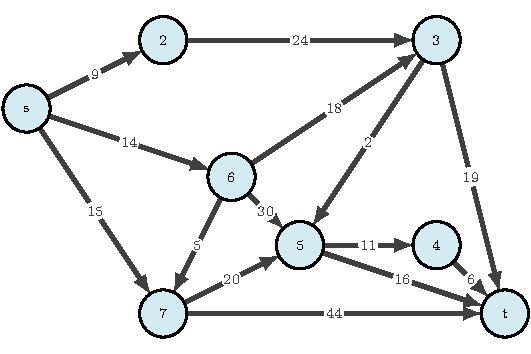
\includegraphics[height=.6\textheight]{fig/ordinal-0.pdf}

        Ordre topologique : $s,6,7,2,3,5,4,t$
    \end{center}
\end{frame}

\begin{frame}{Itérations de l'algorithme : traitement de $s$}
    \begin{center}
        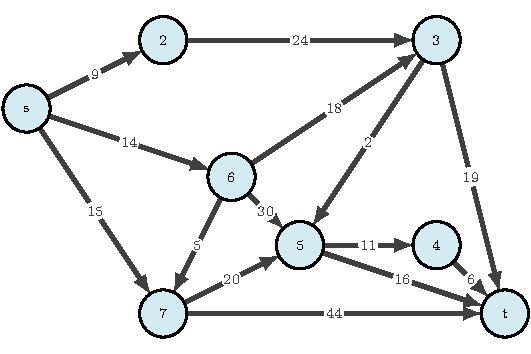
\includegraphics[height=.6\textheight]{fig/ordinal-0.pdf}      
    \begin{tabular}{c|cccccccc}
        
        sommet & s       &2      &7      &6      &5      &3      &4      &t      \\
        \hline
        \texttt{pred} & &       &       &       &       &       &       &       \\
        \texttt{dist} & 0       &inf    &inf    &inf    &inf    &inf    &inf    &inf    \\
    \end{tabular}
\end{center}
\end{frame}

\begin{frame}{Itérations de l'algorithme : traitement de $6$}
    \begin{center}
        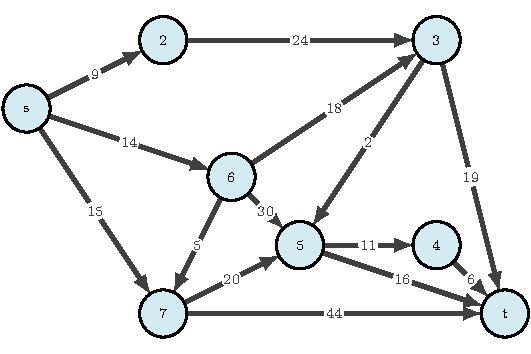
\includegraphics[height=.6\textheight]{fig/ordinal-0.pdf}      
    \begin{tabular}{c|cccccccc}
        
        sommet & s       &2      &7      &6      &5      &3      &4      &t      \\
        \hline
        \texttt{pred} & &       &       &s      &       &       &       &       \\
        \texttt{dist} & 0       &inf    &inf    &14     &inf    &inf    &inf    &inf    \\
    \end{tabular}
\end{center}
\end{frame}

\begin{frame}{Itérations de l'algorithme : traitement de $7$}
    \begin{center}
        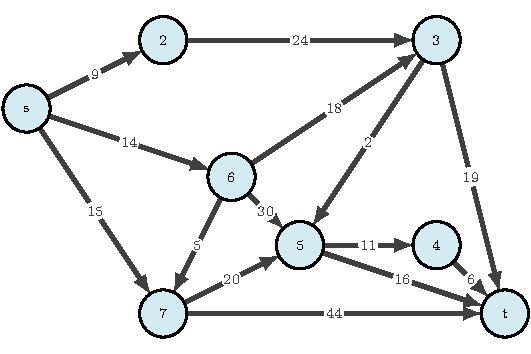
\includegraphics[height=.6\textheight]{fig/ordinal-0.pdf}      
    \begin{tabular}{c|cccccccc}
        
        sommet & s       &2      &7      &6      &5      &3      &4      &t      \\
        \hline
        \texttt{pred} & &       &s      &s      &       &       &       &       \\
        \texttt{dist} & 0       &inf    &15     &14     &inf    &inf    &inf    &inf    \\
    \end{tabular}
\end{center}
\end{frame}

\begin{frame}{Itérations de l'algorithme : traitement de $2$}
    \begin{center}
        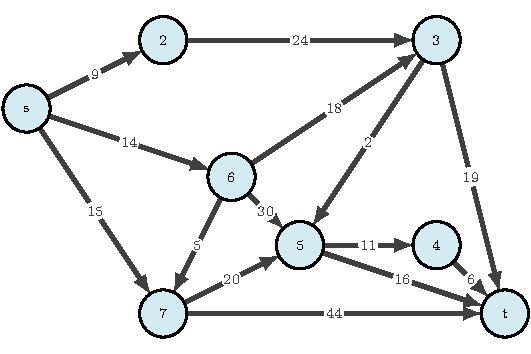
\includegraphics[height=.6\textheight]{fig/ordinal-0.pdf}      
    \begin{tabular}{c|cccccccc}
        
        sommet & s       &2      &7      &6      &5      &3      &4      &t      \\
        \hline
        \texttt{pred} & &s      &s      &s      &       &       &       &       \\
        \texttt{dist} & 0       &9      &15     &14     &inf    &inf    &inf    &inf    \\
    \end{tabular}
\end{center}
\end{frame}

\begin{frame}{Itérations de l'algorithme : traitement de $3$}
    \begin{center}
        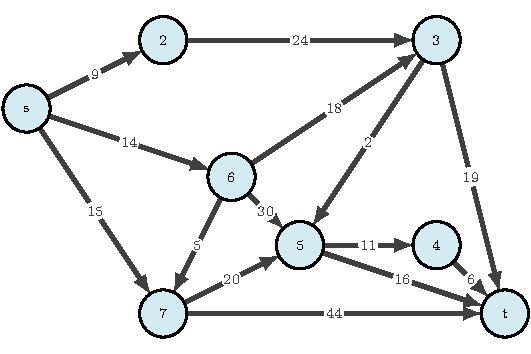
\includegraphics[height=.6\textheight]{fig/ordinal-0.pdf}      
    \begin{tabular}{c|cccccccc}
        
        sommet & s       &2      &7      &6      &5      &3      &4      &t      \\
        \hline
        \texttt{pred} & &s      &s      &s      &       &6      &       &       \\
        \texttt{dist} & 0       &9      &15     &14     &inf    &32     &inf    &inf    \\
    \end{tabular}
\end{center}
\end{frame}

\begin{frame}{Itérations de l'algorithme : traitement de $5$}
    \begin{center}
        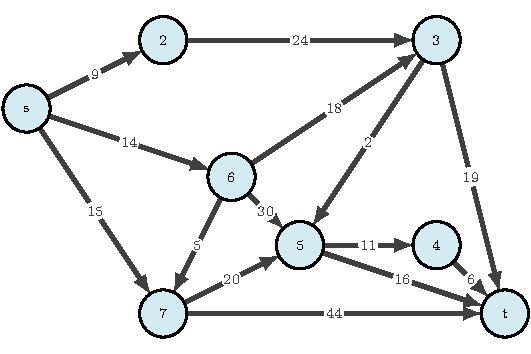
\includegraphics[height=.6\textheight]{fig/ordinal-0.pdf}      
    \begin{tabular}{c|cccccccc}
        
        sommet & s       &2      &7      &6      &5      &3      &4      &t      \\
        \hline
        \texttt{pred} & &s      &s      &s      &3      &6      &       &       \\
        \texttt{dist} & 0       &9      &15     &14     &34     &32     &inf    &inf    \\
    \end{tabular}
\end{center}
\end{frame}

\begin{frame}{Itérations de l'algorithme : traitement de $4$}
    \begin{center}
        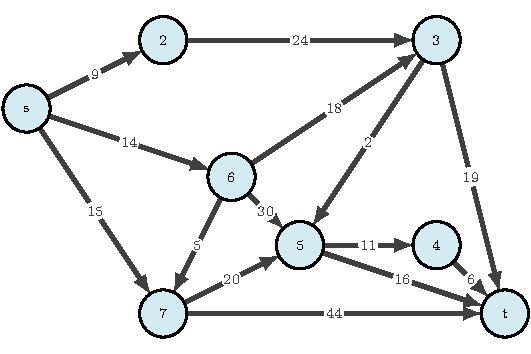
\includegraphics[height=.6\textheight]{fig/ordinal-0.pdf}      
    \begin{tabular}{c|cccccccc}
        
        sommet & s       &2      &7      &6      &5      &3      &4      &t      \\
        \hline
        \texttt{pred} & &s      &s      &s      &3      &6      &5      &       \\
        \texttt{dist} & 0       &9      &15     &14     &34     &32     &45     &inf    \\
    \end{tabular}
\end{center}
\end{frame}

\begin{frame}{Itérations de l'algorithme : traitement de $t$}
    \begin{center}
        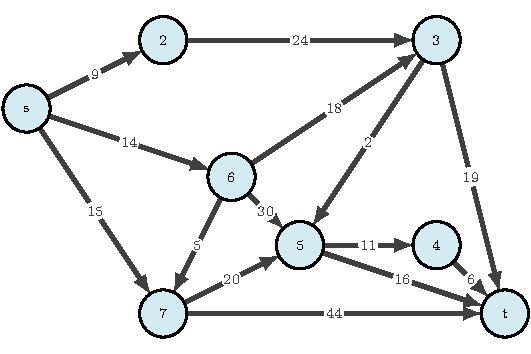
\includegraphics[height=.6\textheight]{fig/ordinal-0.pdf}      
    \begin{tabular}{c|cccccccc}
        
        sommet & s       &2      &7      &6      &5      &3      &4      &t      \\
        \hline
        \texttt{pred} & &s      &s      &s      &3      &6      &5      &5      \\
        \texttt{dist} & 0       &9      &15     &14     &34     &32     &45     &50     \\
    \end{tabular}
\end{center}
\end{frame}


\begin{frame}{Algorithme de Dijkstra}
    \begin{itemize}
        \item On autorise que le graphe contienne des cycles
        \item On se restreint à un \textbf{graphe sans poids négatifs}
        \item Idée : on construit progressivement un ensemble $S$ qui contient les sommets dont nous aurons déjà calculé la distance minimale 
        \item En choisissant à chaque itération un nouveau sommet dont le coût d'accès est minimal qu'on ajoute dans $S$, cette propriété est conservée et on va mettre à jour \texttt{pred} et \texttt{dist} pour les autres sommets
        \item Note : l'algorithme de Dijkstra ressemble fortement à l'algorithme de \prim
    \end{itemize}
\end{frame}

\begin{frame}[fragile]
    \frametitle{Algorithme}
    \begin{algorithmic}[1]
        \Function{Dijkstra}{$G,s$}
            \State dist \gets [0,$\infty$,...,$\infty$]
            \State $P$ \gets $S$, $T$ \gets $\{\}$
            \While{$T$ non vide}
                \State Choisir $x_0 \in T$ tel que \texttt{dist} minimal
                \State $T$ \gets $T-\{ x_0 \}$, $P$ \gets $P \cup \{ x_0 \}$  
                \For{$j \in \Gamma^+(i)$}
                    \If{dist[i]+c(i,j) < dist[j]}
                        \State dist[j] \gets dist[i]+c(i,j)
                        \State pred[j] \gets i
                    \EndIf 
                \EndFor
            \EndWhile
        \EndFunction
    \end{algorithmic}
\end{frame}


\begin{frame}{Exemple}
    \begin{center}
        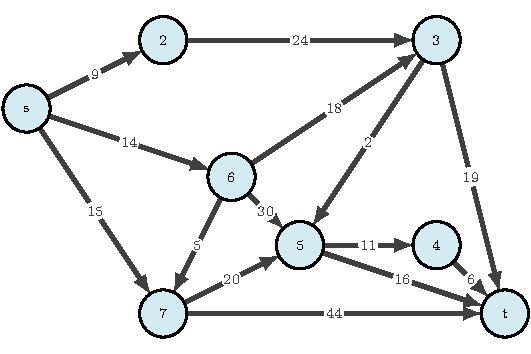
\includegraphics[height=.6\textheight]{fig/dijkstra-0.pdf}

    \end{center}
\end{frame}

\begin{frame}{Itérations de l'algorithme : traitement de $s$}
    \begin{center}
        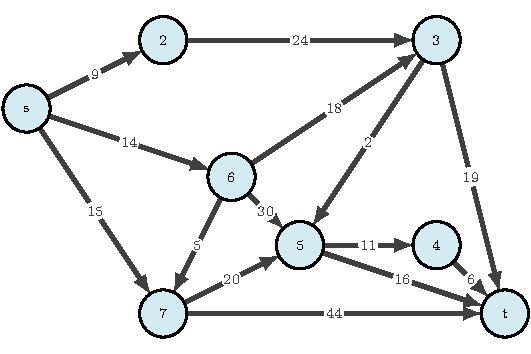
\includegraphics[height=.6\textheight]{fig/dijkstra-0.pdf}      
    \begin{tabular}{c|cccccccc}
      
        & \textbf{s}   &2      &7      &6      &5      &3      &4      &t      \\
        \hline
        \texttt{pred} & &s      &s      &s      &       &       &       &       \\
        \texttt{dist} & 0       &9      &15     &14     &$+\infty$    &$+\infty$    &$+\infty$    &$+\infty$    \\
            \end{tabular}
\end{center}
\end{frame}


\begin{frame}{Itérations de l'algorithme : traitement de $2$}
    \begin{center}
        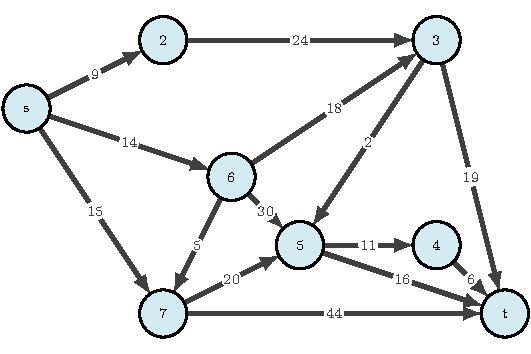
\includegraphics[height=.6\textheight]{fig/dijkstra-0.pdf}      
    \begin{tabular}{c|cccccccc}
      
        & \textbf{s}   &\textbf{2}     &7      &6      &5      &3      &4      &t      \\
        \hline
        \texttt{pred} & &s      &s      &s      &       &2      &       &       \\
        \texttt{dist} & 0       &9      &15     &14     &$+\infty$    &33     &$+\infty$    &$+\infty$    \\
                   \end{tabular}
\end{center}
\end{frame}

\begin{frame}{Itérations de l'algorithme : traitement de $6$}
    \begin{center}
        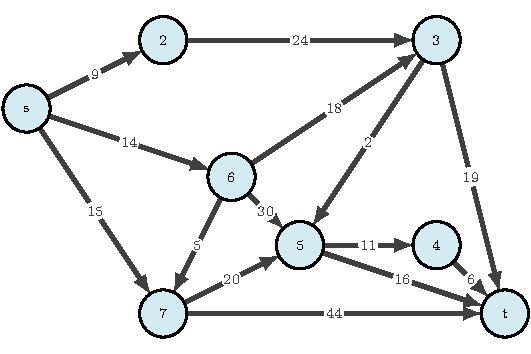
\includegraphics[height=.6\textheight]{fig/dijkstra-0.pdf}      
    \begin{tabular}{c|cccccccc}
      
        & \textbf{s}   &\textbf{2}     &7      &\textbf{6}     &5      &3      &4      &t      \\
        \hline
        \texttt{pred} & &s      &s      &s      &6      &6      &       &       \\
        \texttt{dist} & 0       &9      &15     &14     &44     &32     &$+\infty$    &$+\infty$    \\
                           \end{tabular}
\end{center}
\end{frame}


\begin{frame}{Itérations de l'algorithme : traitement de $7$}
    \begin{center}
        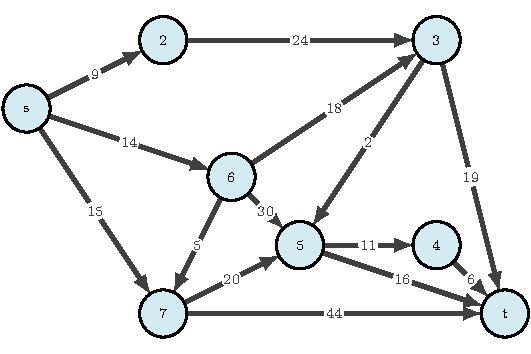
\includegraphics[height=.6\textheight]{fig/dijkstra-0.pdf}      
    \begin{tabular}{c|cccccccc}
      
        & \textbf{s}   &\textbf{2}     &\textbf{7}     &\textbf{6}     &5      &3      &4      &t      \\
        \hline
        \texttt{pred} & &s      &s      &s      &7      &6      &       &7      \\
        \texttt{dist} & 0       &9      &15     &14     &35     &32     &$+\infty$    &59     \\
    \end{tabular}
\end{center}
\end{frame}

\begin{frame}{Itérations de l'algorithme : traitement de $3$}
    \begin{center}
        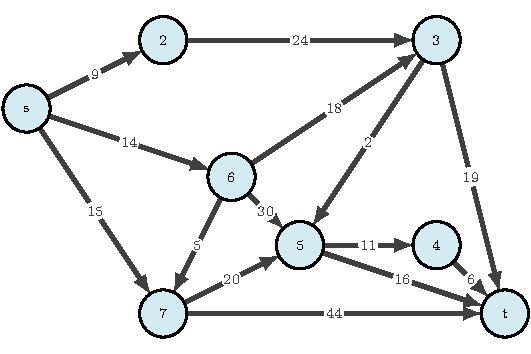
\includegraphics[height=.6\textheight]{fig/dijkstra-0.pdf}      
    \begin{tabular}{c|cccccccc}
      
        & \textbf{s}   &\textbf{2}     &\textbf{7}     &\textbf{6}     &5      &\textbf{3}     &4      &t      \\
        \hline
        \texttt{pred} & &s      &s      &s      &3      &6      &       &3      \\
        \texttt{dist} & 0       &9      &15     &14     &34     &32     &$+\infty$    &51     \\
    \end{tabular}
\end{center}
\end{frame}

\begin{frame}{Itérations de l'algorithme : traitement de $5$}
    \begin{center}
        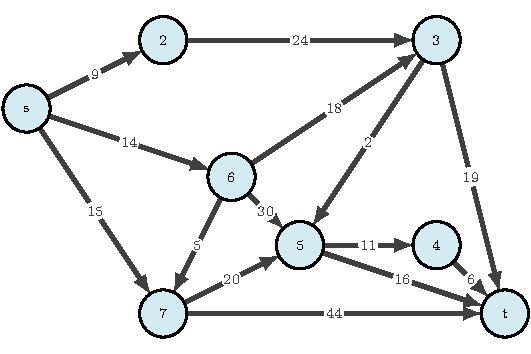
\includegraphics[height=.6\textheight]{fig/dijkstra-0.pdf}      
    \begin{tabular}{c|cccccccc}
      
        & \textbf{s}   &\textbf{2}     &\textbf{7}     &\textbf{6}     &\textbf{5}     &\textbf{3}     &4      &t      \\
        \hline
        \texttt{pred} & &s      &s      &s      &3      &6      &5      &5      \\
        \texttt{dist} & 0       &9      &15     &14     &34     &32     &45     &50     \\
            \end{tabular}
\end{center}
\end{frame}


\begin{frame}{Itérations de l'algorithme : traitement de $4$}
    \begin{center}
        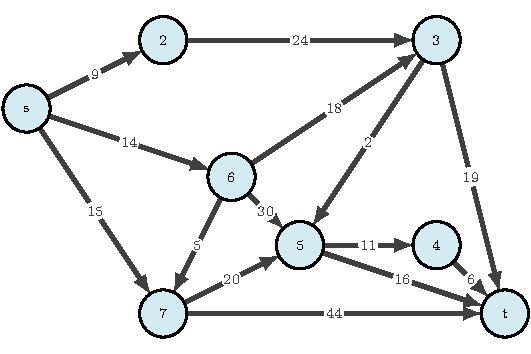
\includegraphics[height=.6\textheight]{fig/dijkstra-0.pdf}      
    \begin{tabular}{c|cccccccc}
      
        & \textbf{s}   &\textbf{2}     &\textbf{7}     &\textbf{6}     &\textbf{5}     &\textbf{3}     &\textbf{4}     &t      \\
        \hline
        \texttt{pred} & &s      &s      &s      &3      &6      &5      &5      \\
        \texttt{dist} & 0       &9      &15     &14     &34     &32     &45     &50     \\
                \end{tabular}
\end{center}
\end{frame}

\begin{frame}{Fin de l'algorithme}
    \begin{center}
        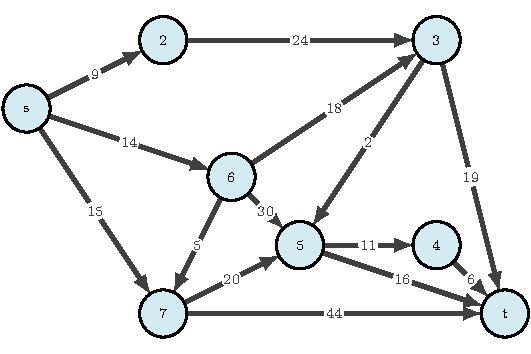
\includegraphics[height=.6\textheight]{fig/dijkstra-0.pdf}      
    \begin{tabular}{c|cccccccc}
      
        & \textbf{s}   &\textbf{2}     &\textbf{7}     &\textbf{6}     &\textbf{5}     &\textbf{3}     &\textbf{4}     &\textbf{t}     \\
        \hline
        \texttt{pred} & &s      &s      &s      &3      &6      &5      &5      \\
        \texttt{dist} & 0       &9      &15     &14     &34     &32     &45     &50     \\
                        \end{tabular}
\end{center}
\end{frame}





%TODO ajouter un exemple Dijkstra avec des cycles 


\begin{frame}{Comparaison des algorithmes}
    \begin{itemize}
        \item Algorithme ordinal 
        \begin{itemize}
            \item pour les graphes acycliques 
            \item Coût en ${\cal O}(n+m)$
        \end{itemize}
        \item Algorithme de Dijkstra 
        \begin{itemize}
            \item pour les graphes sans poids négatifs 
            \item coût ${\cal O}(m \log n + n \log n)$
            \item coût pour une implémentation inspirée de Prim avec une file de priorité sous forme de tas binaire (i.e. pas l'implémentation vue dans le cours)
        \end{itemize}
        \item Reste à voir un algorithme plus général : l'algorithme de Bellman 
    \end{itemize}
\end{frame}

% on passe à l'algorithme de Bellman 

\begin{frame}{Algorithme de Bellman}
    \begin{itemize}
        \item Hypothèse : le graphe ne contient pas de circuit absorbant
        \item Idée : Par rapport à l'algorithme de Dijkstra, on remet en cause tous les chemins à chaque itération 
        \item Justification : variante de l'algorithme Floyd-Warshall sur la fermeture transitive (vu en TD)
        \item Coût : typiquement en ${\cal O}(n^3)$ mais une version optimisée ramène sa complexité à ${\cal O}(nm)$
    \end{itemize}
\end{frame}

\begin{frame}[fragile]
    \frametitle{Algorithme}
    \begin{algorithmic}
        \Function{Bellman}{$G,s$}
            \State dist \gets [0,$\infty$,...,$\infty$]
            \For{$m \in \{1,...,n-2\}$} 
                \For{$x \in S$} 
                    \State dist[$x$] = $\min [ \mathsf{dist}(x) , \min_{y \neq x} [ \mathsf{dist}(y) + c(y,x)]]$ 
                \EndFor
            \EndFor 
            \EndFunction        
    \end{algorithmic}
\end{frame}

\begin{frame}{Exemple}
    \begin{center}
        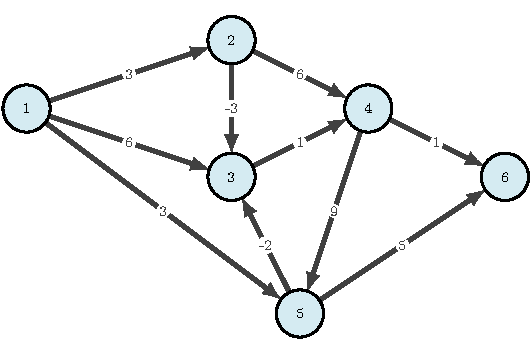
\includegraphics[height=.6\textheight]{fig/bellman-0.pdf}

    \end{center}
\end{frame}

\begin{frame}{Itérations de l'algorithme : itération 1}
    \begin{center}
        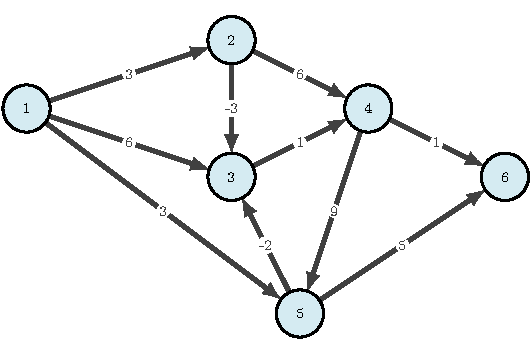
\includegraphics[height=.6\textheight]{fig/bellman-0.pdf}      
    \begin{tabular}{c|cccccc}
      
        & 1    &2      &3      &4      &5      &6      \\
        \hline
        \texttt{pred} & &1      &1      &       &1      &       \\
        \texttt{dist} & 0       &3      &6      &inf    &3      &inf    \\

    \end{tabular}
\end{center}
\end{frame}

\begin{frame}{Itérations de l'algorithme : itération 2}
    \begin{center}
        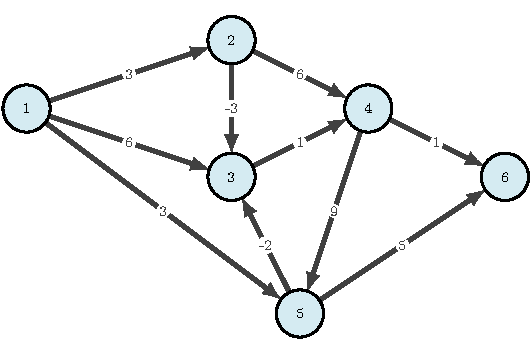
\includegraphics[height=.6\textheight]{fig/bellman-0.pdf}      
    \begin{tabular}{c|cccccc}
      
        & 1    &2      &3      &4      &5      &6      \\
        \hline
        \texttt{pred} & &1      &5      &3      &1      &5           \\
        \texttt{dist} & 0       &3      &1      &7      &3      &8      \\
        
    \end{tabular}
\end{center}
\end{frame}

\begin{frame}{Itérations de l'algorithme : itération 3}
    \begin{center}
        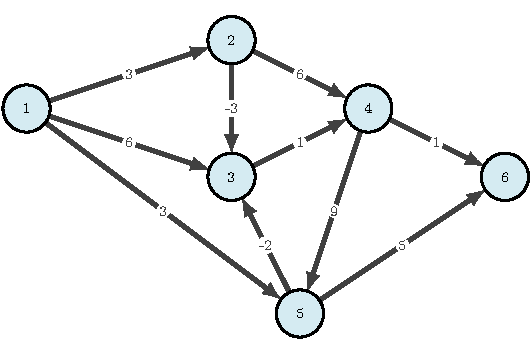
\includegraphics[height=.6\textheight]{fig/bellman-0.pdf}      
    \begin{tabular}{c|cccccc}
      
        & 1    &2      &3      &4      &5      &6      \\
        \hline
        \texttt{pred} & &1      &2      &3      &1      &5      \\
        \texttt{dist} & 0       &3      &0      &2      &3      &8      \\
            \end{tabular}
\end{center}
\end{frame}

\begin{frame}{Itérations de l'algorithme : itération 4}
    \begin{center}
        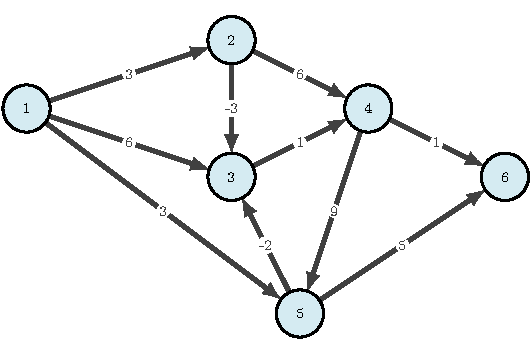
\includegraphics[height=.6\textheight]{fig/bellman-0.pdf}      
    \begin{tabular}{c|cccccc}
      
        & 1    &2      &3      &4      &5      &6      \\
        \hline
        \texttt{pred} & &1      &2      &3      &1      &4      \\
        \texttt{dist} & 0       &3      &0      &1      &3      &3      \\
                    \end{tabular}
\end{center}
\end{frame}


\begin{frame}{Itérations de l'algorithme : itération 5}
    \begin{center}
        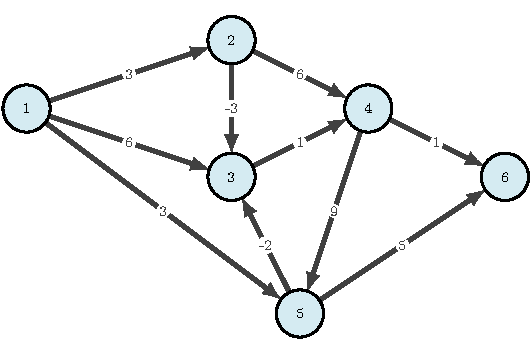
\includegraphics[height=.6\textheight]{fig/bellman-0.pdf}      
    \begin{tabular}{c|cccccc}
      
        & 1    &2      &3      &4      &5      &6      \\
        \hline
        \texttt{pred} & &1      &2      &3      &1      &4     \\
        \texttt{dist} & 0       &3      &0      &1      &3      &2 \\                    \end{tabular}
\end{center}
\end{frame}






\begin{frame}[fragile]
    \frametitle{Version matricielle de l'algorithme de Bellman}
    \begin{itemize}
        \item Si on utilise une représentation sous forme de matrice d'adjacence $m_{i,j}$, l'algorithme de Bellman s'écrit alors sous forme matricielle 
    \end{itemize}
    \begin{algorithmic}[1]
        \Function{bellman\_matriciel}{G,s}
        \State $\Pi_{i,j}^0 = \left\{ 
            \begin{array}{l}
                \mbox{pondération de l'arc s'il existe} \\
                0\mbox{ si } i=j \\
                +\infty \mbox{ sinon}
            \end{array}
        \right.$
        \For{$m \in {1,...,n}$} 
            \For{$i \in {1,...,n}$}
                \For{$j \in {1,...,n}$}
                    \State $\Pi_{i,j}^m = \min \left[\Pi_{i,j}^{m-1}, \Pi_{i,m}^{m-1} + \Pi_{m,j}^{m-1} \right] $
                \EndFor
            \EndFor
        \EndFor
        \EndFunction
    \end{algorithmic}
\end{frame}

% TODO : ça vaut la peine d'ajouter un exemple ? 

